\documentclass[UTF8]{ctexart}
\usepackage{ctex}
\usepackage{titlesec}
\usepackage{fancyhdr}
\usepackage{geometry}
\usepackage{listings}
\usepackage{xcolor}
\usepackage{graphicx}
\usepackage{amsmath}  % 提供了高级数学公式环境
\usepackage{amsfonts} % 提供数学字体
\usepackage{amssymb}  % 提供额外的数学符号
\usepackage{float}
\usepackage{caption} % 自定义图片标题
\usepackage{subcaption} % 子图支持
\usepackage{hyperref} % 添加超链接支持
\hypersetup{
    colorlinks=true, % 设置链接颜色
    linkcolor=black,
    urlcolor=blue,
    citecolor=blue
}
\renewcommand\lstlistingname{} % 将标题名称设为空

\geometry{left=1.0in,right=1.0in,top=0.3in,bottom=0.3in}

\pagestyle{fancy}
\fancyhf{} % 清空当前的页眉和页脚
\fancyfoot[C]{\thepage} % 页脚中间显示页码

\ctexset{
    section={%
        format=\raggedright\Large\bfseries,
        afterskip=10pt,
    },
    subsection={%
        format=\raggedright\normalsize,
        afterskip=8pt,
    }
}

\lstset{
	language=Matlab, 
	extendedchars=false,
	basicstyle=\ttfamily\small, % 字体样式和大小
	keywordstyle=\color{blue}, % 关键字颜色
	commentstyle=\color{gray}, % 注释颜色
	stringstyle=\color{red}, % 字符串颜色
	numberstyle=\tiny\color{gray}, % 行号样式
	frame=single, % 代码框
	breaklines=true, % 自动换行
	captionpos=b % 标题位置
	showspaces=true, showstringspaces=false
	numbers=none
}


\begin{document}

\title{\vspace{0cm}基于总变差(TV)模型图像修复的PDE方程推导以及算法实现}
\author{A类\\韩霈霆 2234412817 贡献率25\%\\程远 2234412848 贡献率25\%\\李梓臻 2233611637 贡献率25\%\\ 吴文正 2234412851 贡献率25\%}


\date{}
\maketitle
\begin{figure}[H]
    \centering
    % 测试图像
    \begin{subfigure}[b]{0.3\textwidth}
        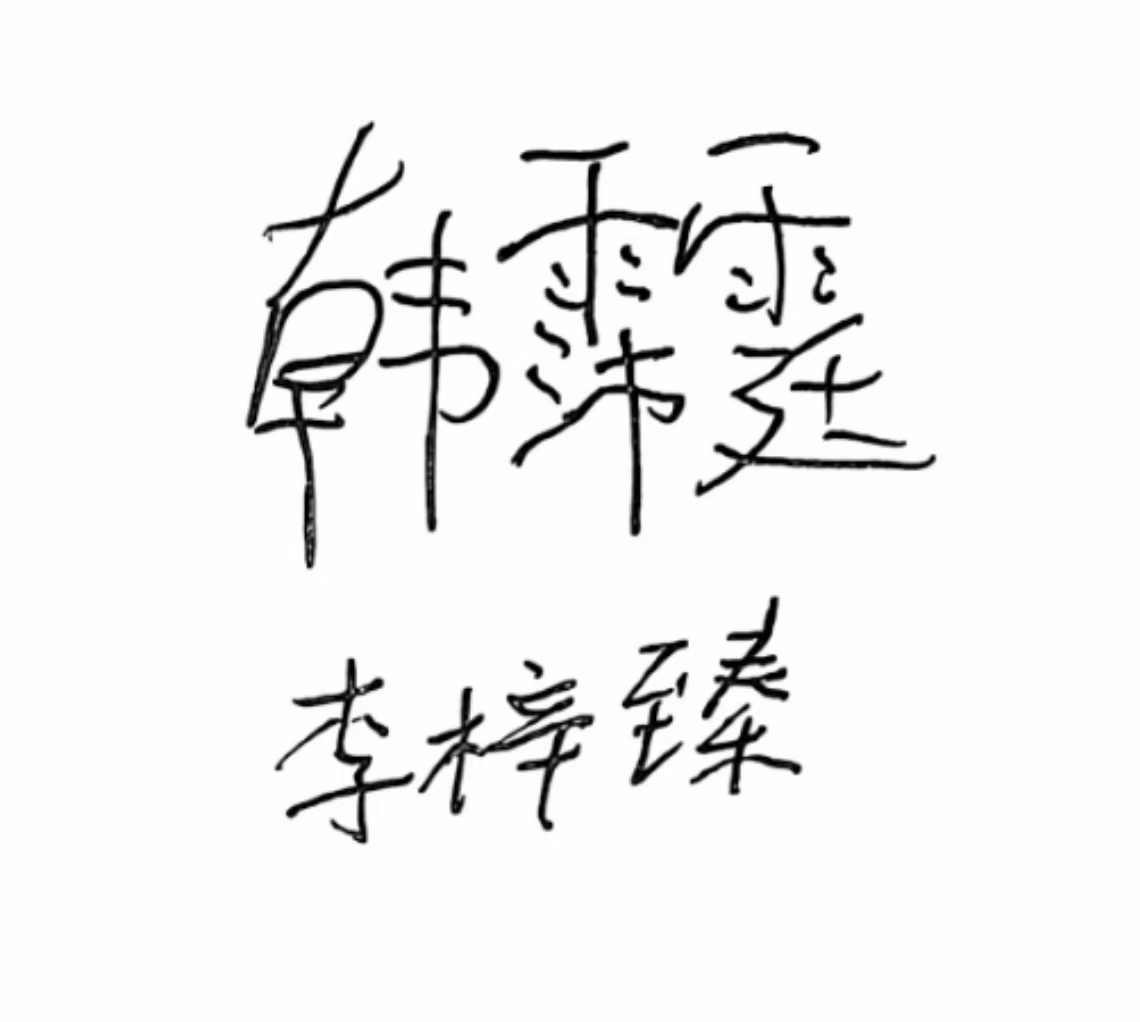
\includegraphics[width=\textwidth]{hpt_lzz.jpg} % 替换为测试图 2 的路径
    \end{subfigure}
    \hfill
    \begin{subfigure}[b]{0.3\textwidth}
        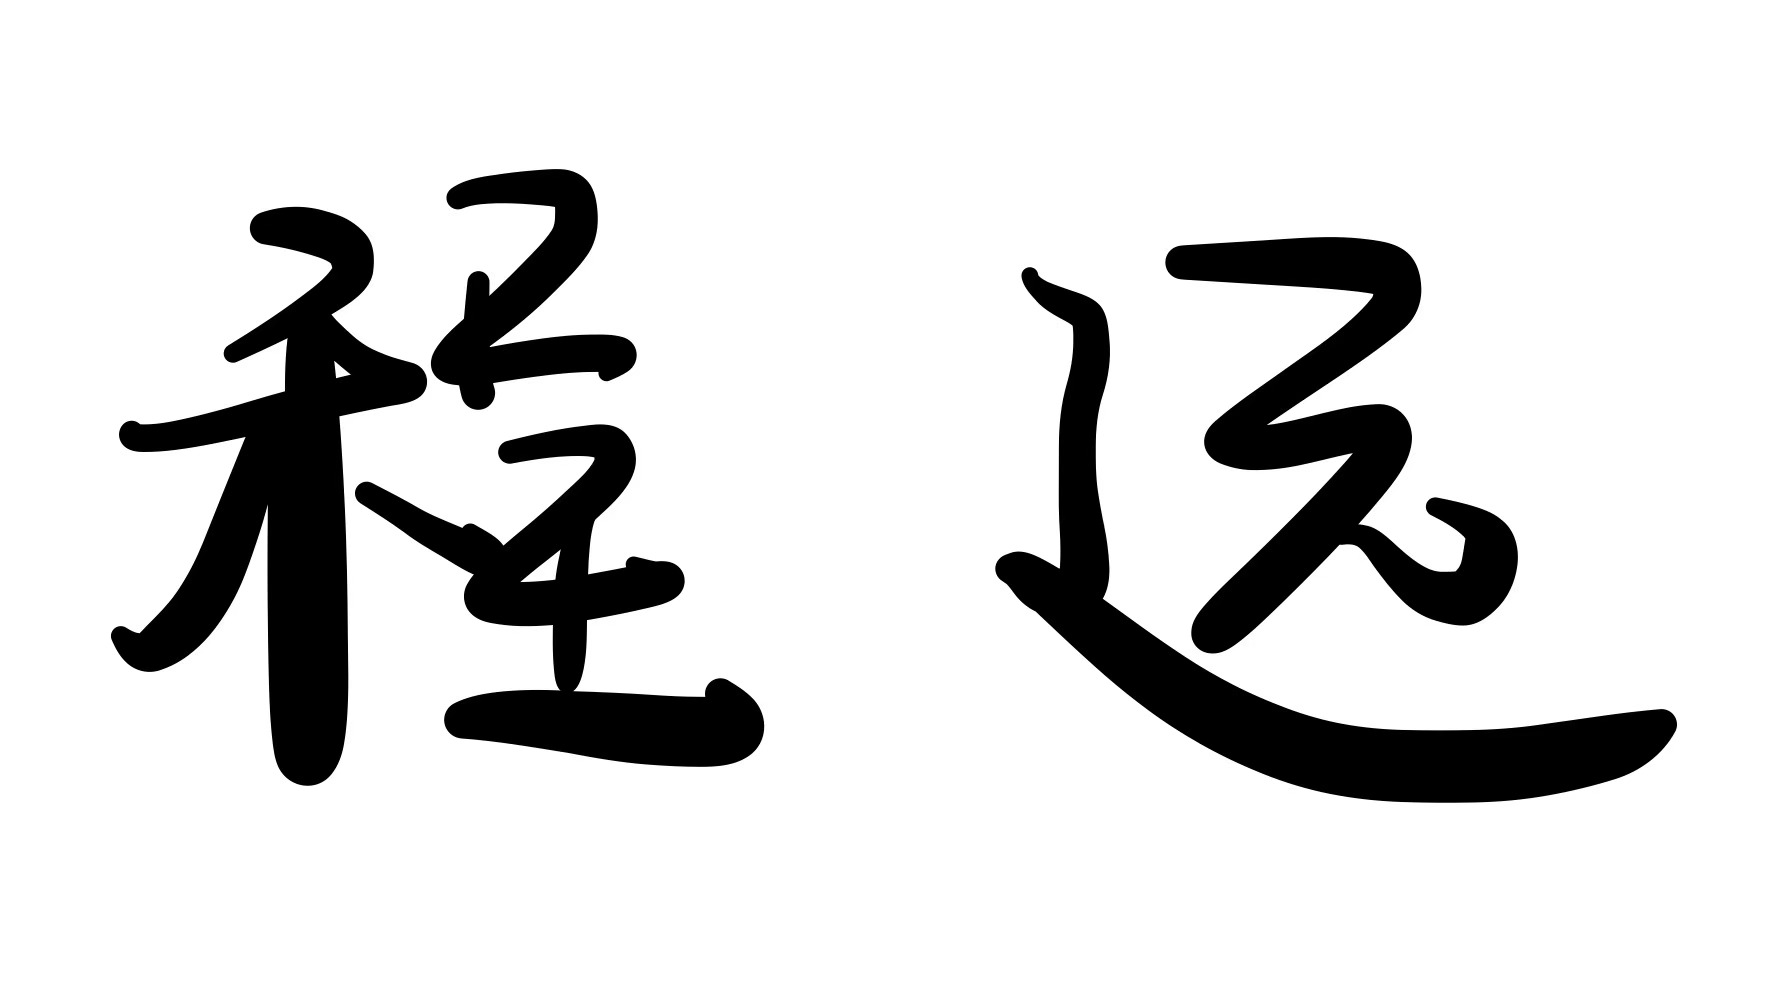
\includegraphics[width=\textwidth]{cy.jpg} % 替换为 Mask 图 2 的路径
    \end{subfigure}
    \hfill
    % 结果图像
    \begin{subfigure}[b]{0.3\textwidth}
        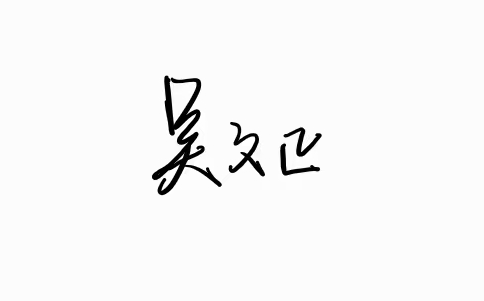
\includegraphics[width=\textwidth]{wwz.png} % 替换为结果图 2 的路径
    \end{subfigure}
\end{figure}
\tableofcontents
\newpage
\section{问题引出}
总变差(TV)是一种基于图像梯度的正则化方法,最早是由数学家Rudin, Osher 和 Fatemi在1992年提出的。他们提出的TV模型最初是用于图像去噪的,
目的是通过最小化图像的总变差来去除噪声,同时保留图像的边缘信息。他们最初提出的公式如下:
\[\min_u \int |\nabla u| \, dx \quad \text{subject to} \quad u = u_0 \quad \text{on known pixels},\]
其中\( u \) 是去噪后的图像,\( u_0 \) 是带噪图像,\( \nabla u \) 是图像 \( u \) 的梯度。
总变差模型的核心思想是,通过惩罚图像的梯度来平滑图像,从而去除图像中的噪声或不必要的细节。此模型的目标是最小化图像的梯度积分,而不是直接最小化图像像素的差异。
然而,这种方法的一个先天缺点是它可能会过度平滑图像,导致细节丢失,尤其是在平滑区域和边缘之间的过渡处。与此同时,在修复过程中,过度依赖梯度信息可能会导致边缘过于硬化或产生伪影。
我们查阅论文发现,为了解决这个问题,研究者们引入了数据一致项$E_{\text{data}}(u) = \int_E |u - u^0|^2 \, dx \, dy$,得到了TV模型修复算法需要优化的泛函:
\[J_{\lambda}[u] = \int_{E \cup D} |\nabla u| \, dx \, dy + \frac{\lambda}{2} \int_{E} |u - u^0|^2 \, dx \, dy\]
式中$D$为待修复图像区域,$E$为由已知像素组
成的$D$的外邻域,$u^0$为$E$内被白噪声污染的原始图
像,$\nabla u$为$u(x,y)$的梯度,$\nabla \cdot$ 表示散度算子。对该泛函的优化过程(即最小化)即为图像修复的过程。

\section{PDE方程求解}
\subsection{应用变分法}
为了最小化 \( J_\lambda[u] \),我们需要通过变分法,求解使 $J_\lambda[u]$ 取得极小值的 $u$。根据变分法的基本理论,满足极值的 $u$ 必须满足对应的 Euler-Lagrange 方程。
Euler-Lagrange 方程的第一项 $\int_{E \cup D} |\nabla u| \, dx \, dy$ 是对图像梯度的总变分,其变分为:
\[
\delta \int_{E \cup D} |\nabla u| \, dx \, dy = \int_{E \cup D} \nabla \cdot \left( \frac{\nabla u}{|\nabla u|} \right) \delta u \, dx \, dy
\]
其中,$\nabla \cdot$ 表示散度算子,$\frac{\nabla u}{|\nabla u|}$ 是梯度的单位方向向量。
第二项 $\frac{\lambda}{2} \int_{E} |u - u^0|^2 \, dx \, dy$ 是数据保留项,其变分为:
\[
\delta \left( \frac{\lambda}{2} \int_{E} |u - u^0|^2 \, dx \, dy \right) = \int_{E} \lambda (u - u^0) \delta u \, dx \, dy
\]
将两部分的变分结合并令其等于零,可得 Euler-Lagrange 方程:
\[
-\nabla \cdot \left( \frac{\nabla u}{|\nabla u|} \right) + \lambda_e (u - u^0) = 0
\]
其中:
\[
\lambda_e =
\begin{cases}
\lambda, & (x, y) \in E \\
0, & (x, y) \in D
\end{cases}
\]
方程第一项 $-\nabla \cdot \left( \frac{\nabla u}{|\nabla u|} \right)$ 描述了图像在不同梯度下的扩散速度,即梯度大的地方扩散较慢,梯度小的地方扩散较快,从而确保了修复的稳定性,保持图像的边缘信息。
第二项 $\lambda_e (u - u^0)$ 描述了已知区域 $E$ 中数据的约束条件,使修复后的图像尽量接近原始已知数据。这一项可以被视为一个约束或惩罚项,
目标是最小化 $u$ 和 $u^0$ 之间的平方误差。在区域 $E$ 中,如果修复后的灰度值 $u(x, y)$ 偏离了原始已知图像的值 $u^0(x, y)$,那么这一项的值会增大,从而在总泛函 $J_\lambda[u]$ 中引入额外的代价。


\subsection{数值差分方程的推导与解释}

为了求解 Euler-Lagrange 方程 $-\nabla \cdot \left( \frac{\nabla u}{|\nabla u|} \right) + \lambda_e (u - u^0) = 0$,需要对梯度的散度 $\nabla \cdot \left( \frac{\nabla u}{|\nabla u|} \right)$ 进行离散化。由于原始图像 $u^0$ 通常没有解析表达式,因此通过数值方法(如中心差分)近似求解。
首先,我们设待修复点为 $O$,其 3×3 的邻域如图所示,$E, N, W, S$ 是 $O$ 的四个相邻像素点,$e, n, w, s$ 是半像素邻近点。
\begin{figure}[H]
    \centering
    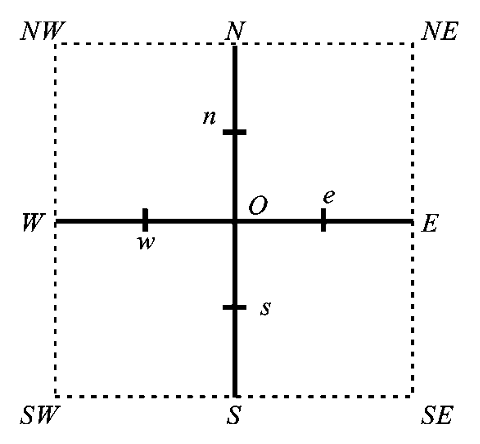
\includegraphics[width=0.4\linewidth]{1.png}
    \label{fig:enter-label}
\end{figure}
记:$\mathbf{v} = \left( v_1, v_2 \right) = \frac{\nabla u}{|\nabla u|}$。那么散度 $\nabla \cdot \mathbf{v}$ 的中心差分近似为:
\[
\nabla \cdot \mathbf{v} = \frac{\partial v_1}{\partial x} + \frac{\partial v_2}{\partial y} \approx \frac{v_1^e - v_1^w}{h} + \frac{v_2^n - v_2^s}{h}
\]
其中 $h$ 为步长,一般取 $h = 1$。

进一步计算半像素点的梯度值。对于 $e$ 点,其梯度值 $v_1^e$ 和 $|\nabla u|_e$ 的计算公式为:
\[
v_1^e = \frac{1}{|\nabla u|_e} \frac{\partial u}{\partial x}\bigg|_e \approx \frac{1}{|\nabla u|_e} \frac{u_E - u_O}{h}
\]
\[
|\nabla u|_e = \frac{1}{h} \sqrt{(u_E - u_O)^2 + \left( \frac{u_{NE} - u_{SE}}{2} \right)^2}
\]
注意到,$\frac{u_{NE} - u_{SE}}{2}$处分母为2,这是因为两点间的距离是$u_E 与 u_O$间距离的两倍,所以我们除2以统一单位距离梯度带来的影响。类似地,可以计算其他半像素点的梯度值 $v_1^w, v_2^n, v_2^s$。将这些值代入散度的表达式,即可得到待修复点 $O$ 的梯度散度的近似值。

图像修复值的计算
根据 Euler-Lagrange 方程:
\[
-\nabla \cdot \left( \frac{\nabla u}{|\nabla u|} \right) + \lambda_e (u - u^0) = 0
\]
通过离散化处理并整理,可以得到以下迭代公式:
\[
\sum_{P \in \Lambda_O} \frac{1}{|\nabla u|_P}(u_O - u_P) + \lambda_e(O)(u_O - u^0_O) = 0
\]
以下是详细的推导过程:

连续形式中的梯度散度项为:
\[
-\nabla \cdot \left( \frac{\nabla u}{|\nabla u|} \right)
\]
在离散化图像中,以像素 $O$ 为中心的邻域 $\Lambda_O = \{E, N, W, S\}$ 表示 $O$ 的四个相邻像素点(东、北、西、南)。
我们定义离散的梯度 $\nabla u$ 为:
   \[
   \frac{\partial u}{\partial x} \approx u_E - u_O, \quad \frac{\partial u}{\partial y} \approx u_N - u_O
   \]
梯度模长的近似计算为:
   \[
   |\nabla u|_P = \sqrt{\left( \frac{\partial u}{\partial x} \right)^2 + \left( \frac{\partial u}{\partial y} \right)^2}
   \]
同理,散度的离散化为:
   \[
   \nabla \cdot \left( \frac{\nabla u}{|\nabla u|} \right) \approx \sum_{P \in \Lambda_O} \frac{1}{|\nabla u|_P} (u_P - u_O)
   \]
   其中 $\frac{1}{|\nabla u|_P}$ 是梯度权重,用于衡量像素间的相对变化。

结合负号,梯度散度项的离散化为:
\[
-\nabla \cdot \left( \frac{\nabla u}{|\nabla u|} \right) \approx \sum_{P \in \Lambda_O} \frac{1}{|\nabla u|_P}(u_O - u_P)
\]
数据保留项 $\lambda_e (u - u^0)$ 通过离散化处理为:
\[
\lambda_e (u - u^0) \to \lambda_e(O) (u_O - u^0_O)
\]
其中:
- $u_O$ 是修复后的当前像素值;
- $u^0_O$ 是已知数据中的像素值;
- $\lambda_e(O)$ 是权重参数,在已知区域 $E$ 内起作用(在待修复区域 $D$ 内 $\lambda_e(O) = 0$)。
将梯度散度项和数据保留项代入 Euler-Lagrange 方程:
\[
\sum_{P \in \Lambda_O} \frac{1}{|\nabla u|_P}(u_O - u_P) + \lambda_e(O)(u_O - u^0_O) = 0
\]
最终离散化公式:
\[
\sum_{P \in \Lambda_O} \frac{1}{|\nabla u|_P}(u_O - u_P) + \lambda_e(O)(u_O - u^0_O) = 0
\]
此公式在离散像素网格上计算修复值,既保护了边缘信息,又保证了已知区域的修复精度。
其中 $\Lambda_O = \{E, N, W, S\}$,为点 $O$ 的四个相邻像素点。

定义权重:
\[
w_P = \frac{1}{|\nabla u|_P}, \quad P \in \Lambda_O
\]
\[
h_{OP} = \frac{w_P}{\sum_{P \in \Lambda_O} w_P + \lambda_e(O)}, \quad h_{OO} = \frac{\lambda_e(O)}{\sum_{P \in \Lambda_O} w_P + \lambda_e(O)}
\]
则 $u_O$ 的更新公式为:
\[
u_O = \sum_{P \in \Lambda_O} h_{OP} u_P + h_{OO} u^0_O
\]
该公式表明:
1. 修复值 $u_O$ 是其邻域像素点值 $u_P$ 和原始已知值 $u^0_O$ 的加权平均。
2. 权重 $h_{OP}$ 和 $h_{OO}$ 的分母中包含邻域内所有像素梯度模的倒数之和 $\sum_{P \in \Lambda_O} w_P$,梯度越大,扩散强度越弱,权重越小。

通过以上的推导,我们将连续的偏微分问题转化为离散的迭代计算问题。通过梯度的各向异性扩散和平滑约束有效图像保留边缘和纹理信息,同时尽量减少修复区域与已知区域之间的突兀感。

\section{代码实现}

根据上述PDE方程的数值解形式,我们设计了一个图像修复程序,对被污染的灰度图像进行修复。代码上述推导的迭代方法,结合梯度信息和权重计算,逐步修复损坏的像素点。

\subsection{代码功能概述}
该代码的主要功能是
读取两幅图像:\texttt{test.jpg} 和 \texttt{mask.jpg}。
\texttt{test.jpg} 是待修复的原始灰度图。
\texttt{mask.jpg} 是用于标记污染区域的掩模图,其中像素值大于 220 的部分被认为是污染区域(纯黑的灰度值为0,代表被污染。纯白的灰度值为255,代表没被污染)。
利用偏微分方程(PDE)中的梯度计算和加权求和方法,逐步修复被污染的图像。


\subsection{代码逐步解析}

读取图像并初始化掩模:使用 \texttt{imread} 读取两幅图像,并将它们转换为灰度图。
将图像转换为 \texttt{double} 类型,以便进行数学运算。
使用逻辑操作 \texttt{>220} 创建掩模图 \texttt{pollute},标记被污染的区域(由于图像压缩算法影响,白色不再纯净,所以我们取像素值大于 220 的部分为 \texttt{true},即没被污染的部分)。
\begin{lstlisting}[language=Matlab]
img = double(rgb2gray(imread('test.jpg')));
pollute = rgb2gray(imread('mask.jpg')) > 220;
[m, n] = size(img);
\end{lstlisting}

初始化待修复图像:遍历图像的每个像素。
如果某像素属于被污染区域(即 \texttt{pollute(i, j) == 0}),将其灰度值设为 0,表示该像素需要修复。
\begin{lstlisting}[language=Matlab]
for i = 1:m
    for j = 1:n
        if pollute(i, j) == 0 % 表示该像素被污染,需要修复
            img(i, j) = 0; 
        end
    end
end
\end{lstlisting}

参数初始化:参数 \texttt{l} 和 \texttt{a} 分别表示正则化项和梯度权重的调节参数:
\begin{itemize}
    \item \texttt{l} 控制已知像素和周围像素的权重分配。
    \item \texttt{a} 用于防止梯度分母为零,确保算法数值稳定性。
\end{itemize}
\texttt{imgn} 是用于存储修复后的图像数据。
\begin{lstlisting}[language=Matlab]
l = 0.2;
a = 0.5;
imgn = img;
\end{lstlisting}

迭代修复过程:外层循环控制修复过程的迭代次数(最多 5000 次)。
内层双循环遍历每个像素,跳过边界像素(防止越界访问)。
仅对被污染的像素(\texttt{pollute(i, j) == 0})进行修复。
\begin{lstlisting}[language=Matlab]
for step = 1:5000 % 迭代次数
    for i = 2:m-1
        for j = 2:n-1
            if pollute(i, j) == 0 % 如果当前像素是被污染的像素,则进行处理
                ...
            end
        end
    end
img = imgn;
end
\end{lstlisting}

梯度计算:分别计算当前像素 $O$ 在四个方向上的梯度(北、东、西、南,分别为 \texttt{un, ue, uw, us})。
梯度由当前像素与邻近像素的差值以及斜对角像素的梯度平均计算得出。
公式中引入的平方根用于计算梯度的模值,表示像素间的强度变化。
\begin{lstlisting}[language=Matlab]
un = sqrt((img(i, j)-img(i-1, j))^2 + ((img(i-1, j-1)-img(i-1, j+1))/2)^2);
ue = sqrt((img(i, j)-img(i, j+1))^2 + ((img(i-1, j+1)-img(i+1, j+1))/2)^2);
uw = sqrt((img(i, j)-img(i, j-1))^2 + ((img(i-1, j-1)-img(i+1, j-1))/2)^2);
us = sqrt((img(i, j)-img(i+1, j))^2 + ((img(i+1, j-1)-img(i+1, j+1))/2)^2);
\end{lstlisting}

权重计算:根据梯度模值计算各方向的权重 \texttt{wn, we, ww, ws}。
引入参数 \texttt{a} 避免梯度过小导致分母接近 0,从而稳定数值计算。
梯度模值越大(即像素差异越显著),对应的权重越小,从而保护图像的边缘信息。这里我们使用平方平均来保证在u项较大时,a的影响能够较好地被忽略。
\begin{lstlisting}[language=Matlab]
wn = 1 / sqrt(un^2 + a^2);
we = 1 / sqrt(ue^2 + a^2);
ww = 1 / sqrt(uw^2 + a^2);
ws = 1 / sqrt(us^2 + a^2);
\end{lstlisting}

修复像素值计算:计算修复权重(\texttt{hon, hoe, how, hos, hoo})。
新的像素值由相邻像素的加权平均值计算得出,体现了梯度扩散的效果。
\begin{lstlisting}[language=Matlab]
hon = wn / ((wn + we + ww + ws) + l);
hoe = we / ((wn + we + ww + ws) + l);
how = ww / ((wn + we + ww + ws) + l);
hos = ws / ((wn + we + ww + ws) + l);
hoo = l / ((wn + we + ww + ws) + l);
imgn(i, j) = hon*img(i-1, j) + hoe*img(i, j+1) + how*img(i, j-1) + hos*img(i+1, j) + hoo*img(i, j);
\end{lstlisting}

更新图像并显示结果:每次迭代完成后,通过 \texttt{imshow} 显示修复结果。
\begin{lstlisting}[language=Matlab]
figure;
imshow(img, []);
\end{lstlisting}

\section{测试图像与结果}

\subsection{第一组测试}

\begin{figure}[H]
    \centering
    % 测试图像
    \begin{subfigure}[b]{0.3\textwidth}
        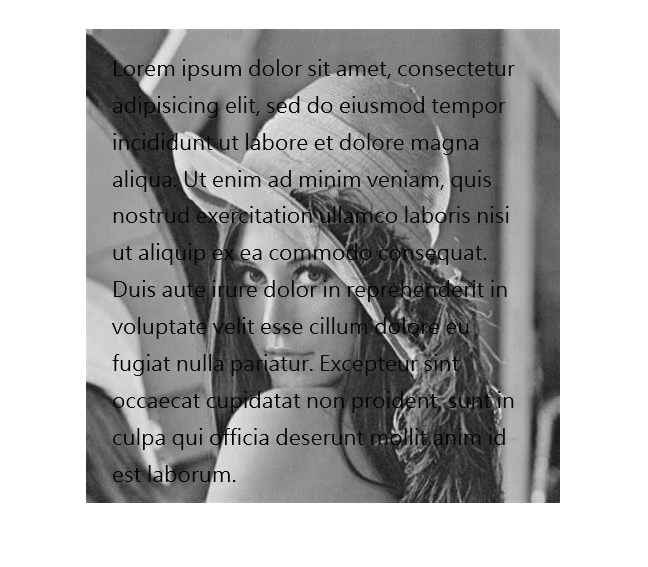
\includegraphics[width=\textwidth]{test.png} % 替换为测试图 1 的路径
        \caption{测试图 1}
        \label{fig:test1}
    \end{subfigure}
    \hfill
    % Mask图像
    \begin{subfigure}[b]{0.3\textwidth}
        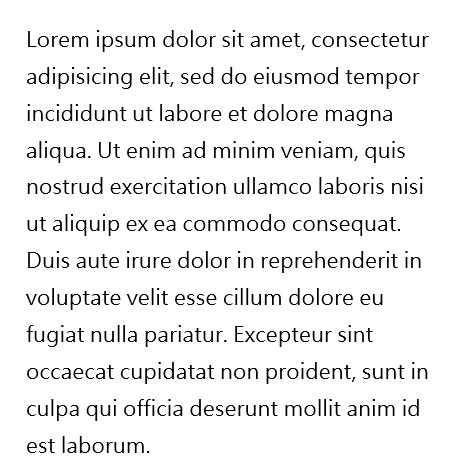
\includegraphics[width=\textwidth]{mask.jpg} % 替换为 Mask 图 1 的路径
        \caption{掩模图 1}
        \label{fig:mask1}
    \end{subfigure}
    \hfill
    % 结果图像
    \begin{subfigure}[b]{0.3\textwidth}
        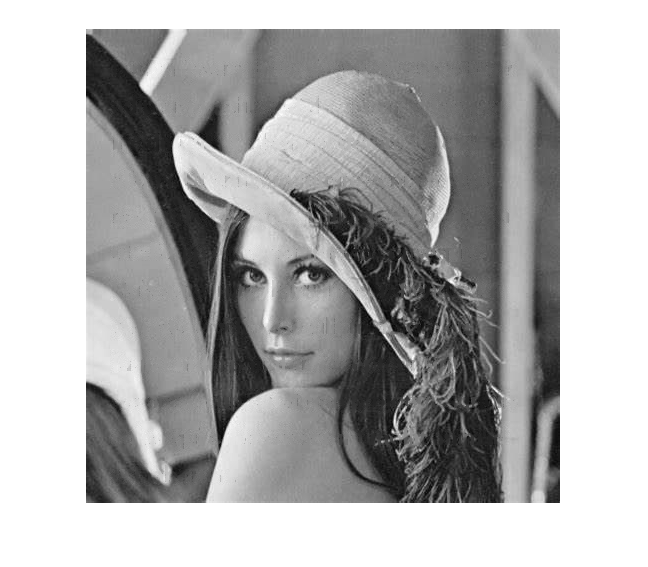
\includegraphics[width=\textwidth]{res.png} % 替换为结果图 1 的路径
        \caption{结果图 1}
        \label{fig:res1}
    \end{subfigure}
    \caption{第一组测试图、掩模图和修复结果}
    \label{fig:group1}
\end{figure}

\subsection{第二组测试}

\begin{figure}[H]
    \centering
    % 测试图像
    \begin{subfigure}[b]{0.3\textwidth}
        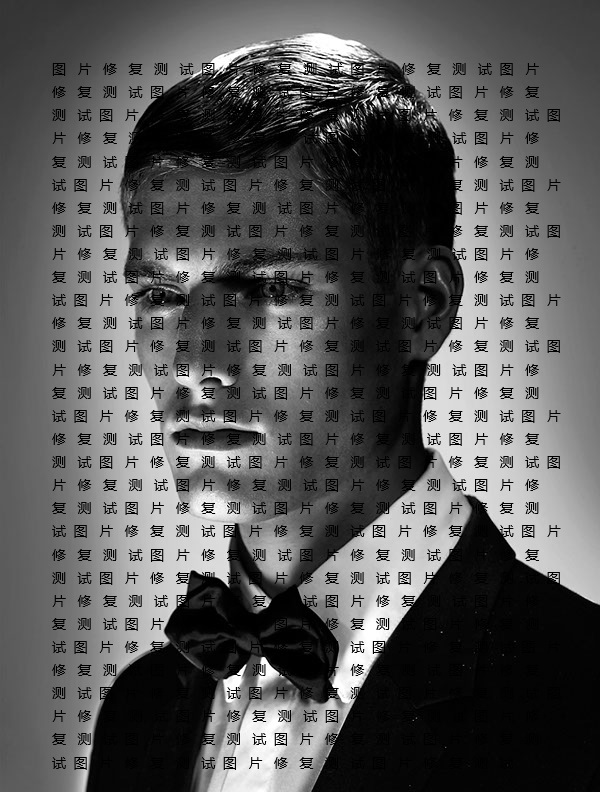
\includegraphics[width=\textwidth]{test2.jpg} % 替换为测试图 2 的路径
        \caption{测试图 2}
        \label{fig:test2}
    \end{subfigure}
    \hfill
    % Mask图像
    \begin{subfigure}[b]{0.3\textwidth}
        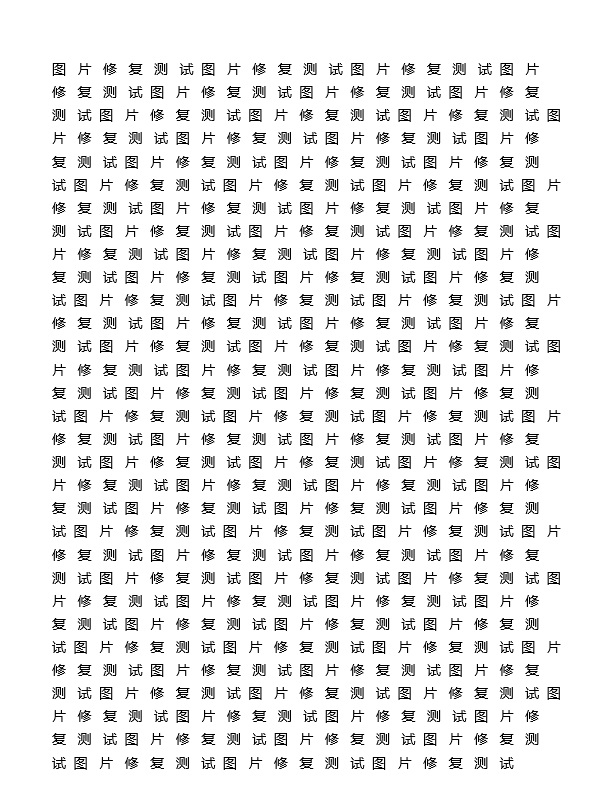
\includegraphics[width=\textwidth]{mask2.jpg} % 替换为 Mask 图 2 的路径
        \caption{掩模图 2}
        \label{fig:mask2}
    \end{subfigure}
    \hfill
    % 结果图像
    \begin{subfigure}[b]{0.3\textwidth}
        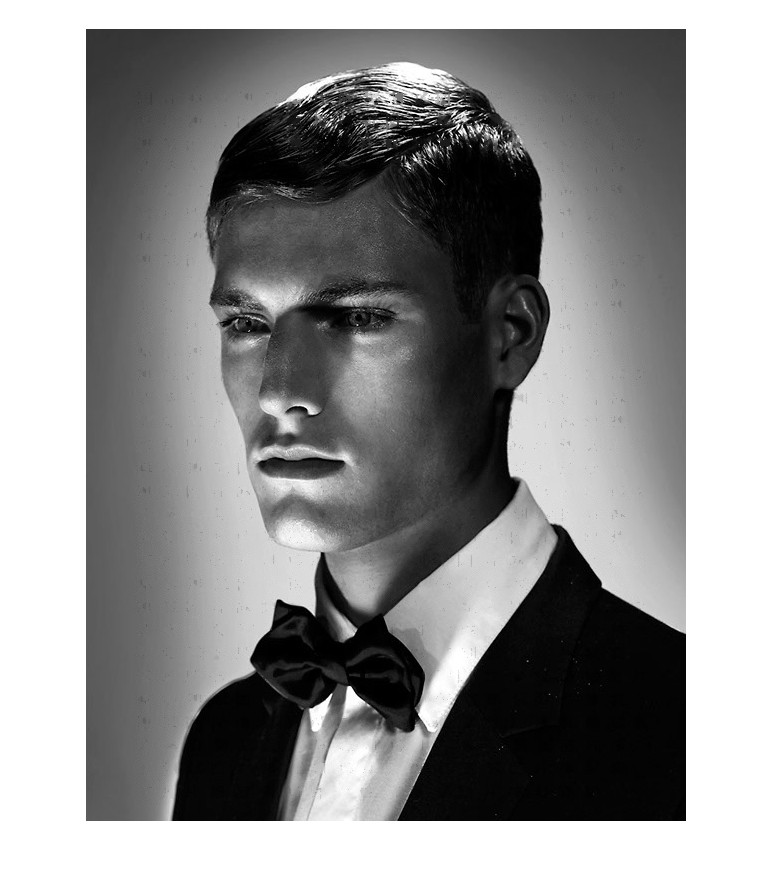
\includegraphics[width=\textwidth]{res2.jpg} % 替换为结果图 2 的路径
        \caption{结果图 2}
        \label{fig:res2}
    \end{subfigure}
    \caption{第二组测试图、掩模图和修复结果}
    \label{fig:group2}
\end{figure}
可以看到,我们的算法较好地保留了图像边缘的信息,并且实现了相当明显与理想的修复效果。

\section{彩色图像修复的创新尝试}
对于彩色图片,我们参考灰色图片思路。先将其分为三个通道,然后分别对三个通道进行修复,之后再将三个通道合并变成一副修复后的图像。
但是修复之后的图像效果明显不如灰度图像。这可能是因为在视觉上,三个通道不是简单的叠加,他们之间是有相互联系的。用拆开再合并的方法没法很好的处理这种联系。
而这种关系是蕴含在rgb三通道这个三维向量中。因此tv模型没法很好地完成彩色图像的修复。
下图是我们使用分别处理三个通道方法的结果。
\begin{figure}[H]
    \centering
    % 测试图像
    \begin{subfigure}[b]{0.3\textwidth}
        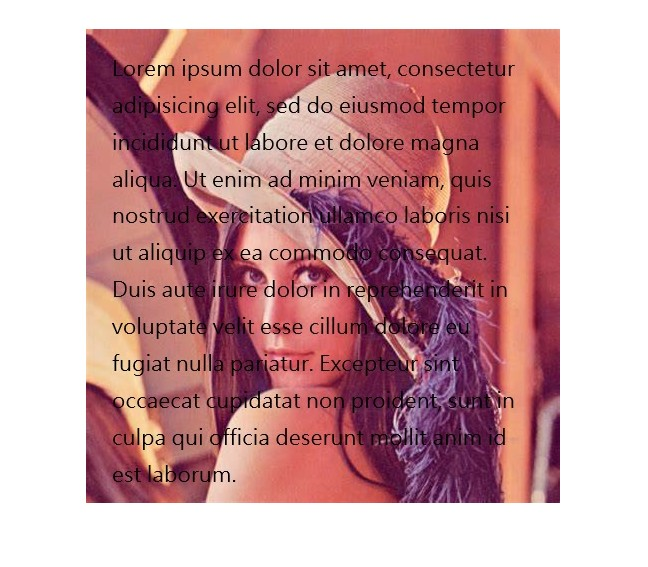
\includegraphics[width=\textwidth]{test3.jpg} % 替换为测试图 2 的路径
        \caption{测试图 3}
        \label{fig:test2}
    \end{subfigure}
    \hfill
    % Mask图像
    \begin{subfigure}[b]{0.3\textwidth}
        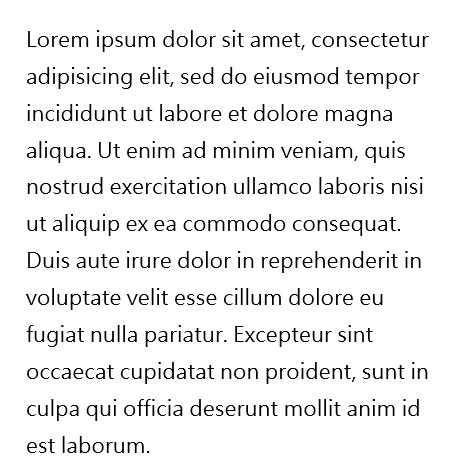
\includegraphics[width=\textwidth]{mask.jpg} % 替换为 Mask 图 2 的路径
        \caption{掩模图 3}
        \label{fig:mask2}
    \end{subfigure}
    \hfill
    % 结果图像
    \begin{subfigure}[b]{0.3\textwidth}
        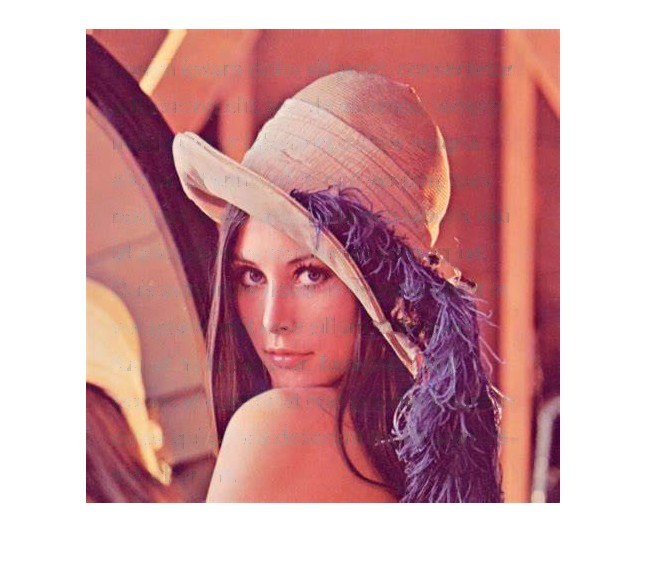
\includegraphics[width=\textwidth]{res3.jpg} % 替换为结果图 2 的路径
        \caption{结果图 3}
        \label{fig:res2}
    \end{subfigure}
    \caption{第三组(彩色)测试图、掩模图和修复结果}
    \label{fig:group2}
\end{figure}

为了解决上述问题,我们在查阅论文后发现可以引入交叉通道梯度,将 RGB 三通道的信息结合起来,以增强算法对彩色图像的修复能力。
传统 TV 算法中,梯度通常定义为单个通道内像素的差异。例如,对于像素点 \((i, j)\),红色通道的梯度为:
\[
\nabla u_R = \left( u_R(i+1, j) - u_R(i, j), \, u_R(i, j+1) - u_R(i, j) \right),
\]
其中 \(u_R\) 表示红色通道。

为了捕捉通道间的颜色变化,我们定义交叉通道梯度:
\[
\nabla u_{RG} = \left( u_R(i, j) - u_G(i, j), \, u_R(i+1, j) - u_G(i+1, j) \right),
\]
\[
\nabla u_{RB} = \left( u_R(i, j) - u_B(i, j), \, u_R(i, j+1) - u_B(i, j+1) \right).
\]

结合通道内和通道间梯度信息,我们定义新的梯度模长:
\[
|\nabla u| = \sqrt{|\nabla u_R|^2 + |\nabla u_G|^2 + |\nabla u_B|^2 + w_{RG} |\nabla u_{RG}|^2 + w_{RB} |\nabla u_{RB}|^2},
\]
其中:
\begin{itemize}
    \item \(w_{RG}\) 和 \(w_{RB}\) 是交叉通道梯度的权重,用于平衡通道内梯度和交叉通道梯度的贡献。
    \item 单通道梯度项(如 \(|\nabla u_R|\))用于保持各通道的局部平滑性。
    \item 交叉通道梯度项(如 \(|\nabla u_{RG}|\))用于增强颜色相关性和边缘信息的描述。
\end{itemize}
在实际修复中,交叉通道梯度的权重 \(w_{RG}\) 和 \(w_{RB}\) 可以根据局部特性动态调整。例如:
\[
w_{RG}(i, j) = \frac{\exp(-|\nabla u_{RG}(i, j)|)}{Z},
\]
其中 \(Z\) 是归一化因子,确保权重的范围在合理区间内。这样可以:
\begin{itemize}
    \item 在高纹理区域(梯度模长较大时),增大交叉通道梯度的权重,以更好地捕捉颜色变化。
    \item 在平滑区域(梯度模长较小时),降低交叉通道梯度的权重,避免过度强调颜色差异。
\end{itemize}

\subsection{结合优先级策略}
在修复过程中,将交叉通道梯度引入优先级的计算中。优先级的定义包括置信度项 \(C(p)\) 和数据项 \(D(p)\):
\[
P(p) = C(p) \cdot D(p).
\]
其中,数据项 \(D(p)\) 可以定义为:
\[
D(p) = |\nabla u(p)| \cdot \left( w_{RG} |\nabla u_{RG}(p)| + w_{RB} |\nabla u_{RB}(p)| \right).
\]
这种设计确保修复时优先考虑颜色变化显著的区域。

\subsection{改进效果}
由于计算机硬件限制,无法处理如此大量的计算,迭代五十步之内效果不明显,而五十步之后matlab崩溃,程序无法完整运行。


\section{结论}
本文引入总变差(TV)模型及其用于图像修复中所需的泛函,应用变分法获得该泛函的极小值条件,即 Euler-Lagrange 方程,并通过数值差分方法对该偏微分方程进行离散化处理,
最终得到了用于图像修复的迭代公式并使用MatLab给出了所得公式的一个实现。经测试,在灰度图像修复方面,我们的算法能够有效地保留图像的边缘信息,并实现较为理想的修复效果。在彩色图像修复方面,
我们尝试了将图像分为三个通道分别进行修复的方法,但效果不如预期。为了解决这一问题,我们引入了交叉通道梯度,将 RGB 三通道的信息结合起来,以增强算法对彩色图像的修复能力。
通过定义新的梯度模长和结合优先级策略,我们的改进方法在理论上能够更好地捕捉颜色变化和边缘信息。然而,由于计算机硬件的限制,我们的算法在处理大规模计算时存在一定的局限性。
在迭代五十步之后,程序无法完整运行。查阅资料发现可以进一步优化该算法的计算效率,或改用效率更高的图像修复方法如深度学习等以提高修复效果和计算性能。
\section{声明}

%放在结论和参考文献部分之间

本次大作业的分工情况为:

吴文正同学主要负责参考文献部分的工作,感谢他对于相关资料的查询与最终参考文献引用部分的整理,为小组的工作提供了充足且可靠的可查阅信息与理论依据;

程远同学主要负责理论学习以及报告主题部分撰写的工作,特别感谢他对于TV模型修复算法等概念、求解方法的学习与阐释,为小组的研究提供了明确的路径指引,并将研究成果进行了清晰的展示;

韩霈霆同学主要负责图像修复程序主体部分编写的工作,特别感谢他对于两种(灰色、彩色)图像修复程序总体框架的搭建与算法的优化,成功地完成小组研究的算法在Matlab编程语言下的实现;

李梓臻同学主要负责图像修复程序的调试运行以及报告的校对修订工作,感谢他对于测试用例的设计与对于程序的调整,以及对于报告中知识性、格式性疏漏的补充和修订,分担了小组工作中的大量琐碎部分。

\begin{thebibliography}{99}
    \bibitem{ref1} 霍俊蓉. 基于偏微分方程的图像修复数值模型[J]. 计算机科学与应用, 2021, 11(8): 2035-2041. doi:10.12677/CSA.2021.118208.
    \bibitem{ref2} 赵颜伟, 李象霖. 一种基于TV模型的快速图像修复算法[J]. 微电子学与计算机, 2009, 26(6): 253-256, 260.
    \bibitem{ref3} 李爱菊, 钮文良. 基于改进Criminisi算法的图像修复[J]. 计算机工程与应用, 2014, 50(18): 167-170.
    \bibitem{ref4} Matlab科研辅导帮. 基于 PDE 算法彩色图像修复附 Matlab 实现[EB/OL]. CSDN, 2023-12-18[2024-12-28].\url{https://blog.csdn.net/m0_60703264/article/details/135352119}.
    \bibitem{ref5} Matlab武动乾坤. 偏微分方程 PDE 图像去噪(含 SNR)[EB/OL]. CSDN, 2023-12-20[2024-12-28].\url{https://blog.csdn.net/KeepingMatlab/article/details/135931557}.
    \bibitem{ref6} Nirvana. 全变分图像去噪算法(TV)[EB/OL]. CSDN, 2021-07-01[2024-12-28].\url{https://blog.csdn.net/weixin_45355387/article/details/118968623}.
\end{thebibliography}

\end{document}